



%\subsection{Simulaciones Médicas}
\begin{frame}{\citetitle{MarcoNuno_Revista_2020_10_00} \footnotemark (1)}
\begin{block}{Problem Description \footnotemark (1)} 
%\begin{columns}
%\begin{column}{0.95\textwidth}
	\begin{itemize}
	\item There are several reviews of applications for diabetes management.

	\item Types of diabetes management apps: blood glucose logging, nutrition databases, carbohydrate
tracking, tracking physical activity and weight, data-sharing and social support, and short messages and reminders.
	\note[item]{Diabetes management apps considered critical factors: patient demographics, technology costs, platform varieties, and ease of use.}
%	\note[item]{One uncommon type of app are those glucose level simulators, which are main based on desktop app or web based app. }
\item Most of the existing glucose levels simulators are Desktops apps or Web-based. There are no glucose level simulators on smartphones. 
	\note[item]{Web-based simulators have as main disadvantage the requirement of Internet connectivity, making the simulator difficult to access in places with connectivity problems.}
	\note[item]{Desktop-based simulators have as main disadvantage the requirement of a Desktop or Laptop PC, making the simulator unavailable to people that does not have a computer.}

\item We proposed an educational mobile assistant application to help support therapy in patients with diabetes
	\end{itemize}
%\end{column}
%\begin{column}{0.05\textwidth}
%\end{column}
%\end{columns}
\end{block} 
\footnotetext[1]{\fullcite{MarcoNuno_Revista_2020_10_00}}
\setcounter{footnote}{0}

\end{frame}

\begin{frame}{\citetitle{MarcoNuno_Revista_2020_10_00} (2)}
\begin{block}{Diabetic Patient Model} 
\begin{columns}
\begin{column}{0.5\textwidth}
\begin{itemize}
%\item Creating an artificial model for a glucose-insulin system for several purposes has been widely explored. The models includes in this app are:
\item The artificial glucose-insulin simulator used in this app has the following modules:
\begin{itemize}
\item Glucose-Insulin Model. 
\note[item]{The Glucose-Insulin Model ... simulates metabolic effects related to glucose regulation.}
\item Insulin model,  
\note[item]{The insulin model ...  describes the subcutaneous insulin uptake pattern after an insulin injection. }
\item Meal Intake model
\note[item]{The meal intake model .... Describes the gastric glucose absorption into the bloodstream by a meal intake represented by its carbohydrates content.}
\item The exercise model.
\note[item]{The excerise model ... estimates the liver’s glycogen reservoir based on the glucose uptake due to exercise intensity, percentage of the maximum oxygen consumption rate. }
\end{itemize}
The app takes as input:
\begin{itemize}
\item Insulin dose parameters 
\note[item]{Incluiding fast and slow action insulins}
\item Meal profile 
 \note[item]{Incluiding carbohydrate grams and meal hours}
\item Excercise quantification
 \note[item]{(Days, hours and intensity)}
\end{itemize}
\end{itemize}

%There are four subsystems, each one corresponds to a previously described model, and their interactions are shown as solid arrows.
\end{column}
\begin{column}{0.5\textwidth}

\begin{center}
     %%%%% this is a minipage, so \textwidth is already adjusted to the size of the column
     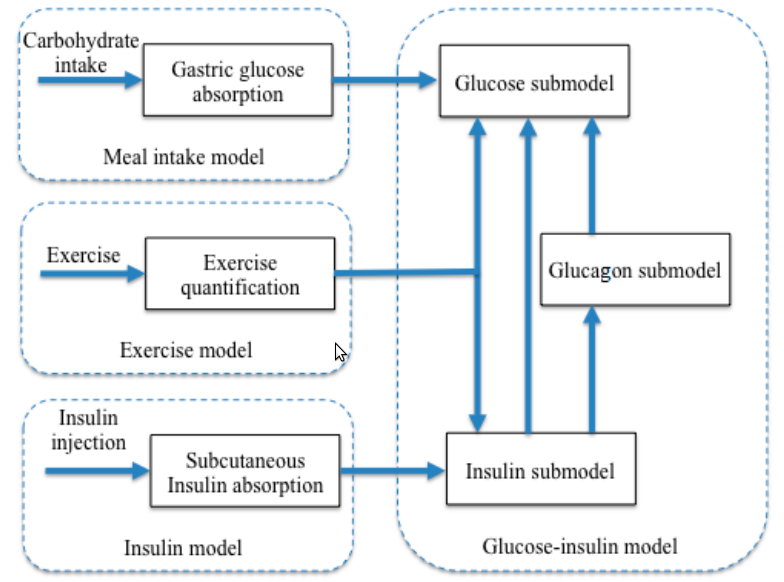
\includegraphics[width=0.99\textwidth]{Figs/Diabetes1}
     \end{center}
     \end{column}
     \end{columns}
\end{block}
\end{frame}


\begin{frame}{\citetitle{MarcoNuno_Revista_2020_10_00} (3)}
\note[item]{The first screen shown the presentation screen of the app.}
\note[item]{The second screen shows a 4-tab apps, where the first tab shows the inputs of the meal model, including meals times and carbohydrate grams per meal.}
\note[item]{The second tab shows the inputs of the insulin model, including both rapid and prolonged insulins, and the dose (units) of each insulin.}
\note[item]{The third tab shows the inputs of the excerise model, including days and hour of the excersise, durations and quantification of the exercise.}
\note[item]{The fourth tab shows the simulation controls, where user can start the simulation and after the finalization, the user can display the glucose consentration plot based on the data input to the models.}

\begin{block}{Mobile app screens (2)} 
\begin{itemize}
\item The proposed app has four tabs (meal, insulin, exercise and simulation)
\end{itemize}
\begin{center}
     \begin{tabular}{ccccc}

\includegraphics[width=0.17\textwidth]{Figs/Pantalla0_AEDMA}     &
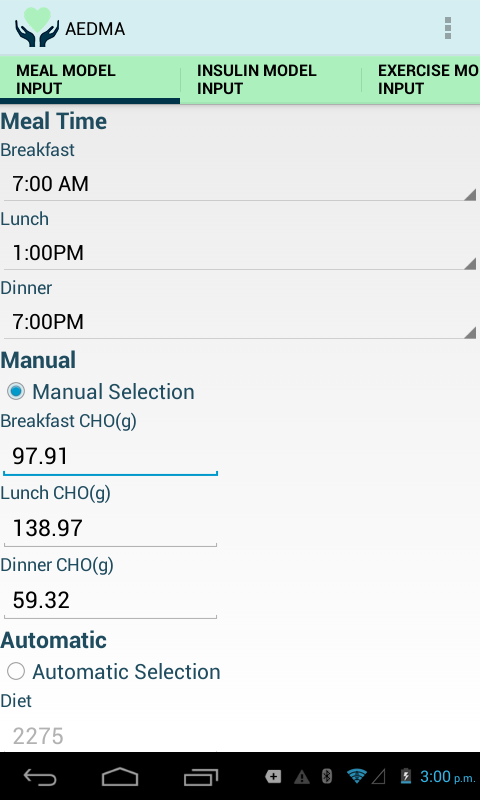
\includegraphics[width=0.17\textwidth]{Figs/Pantalla1_AEDMA}     &
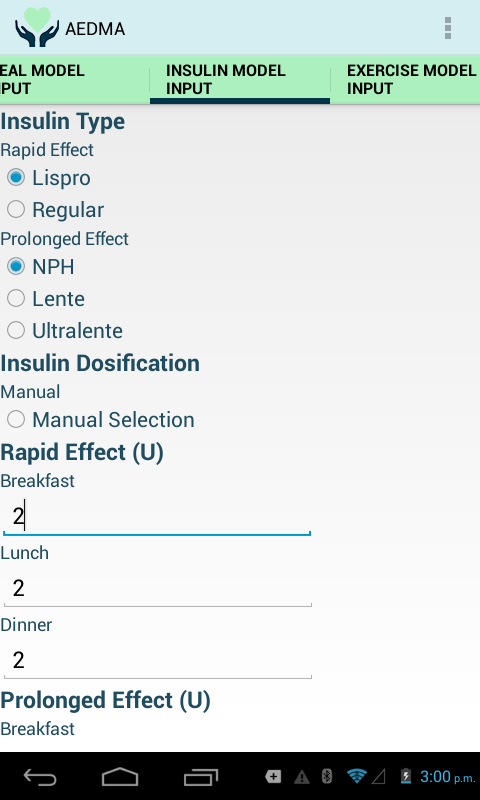
\includegraphics[width=0.17\textwidth]{Figs/Pantalla2_AEDMA}     &
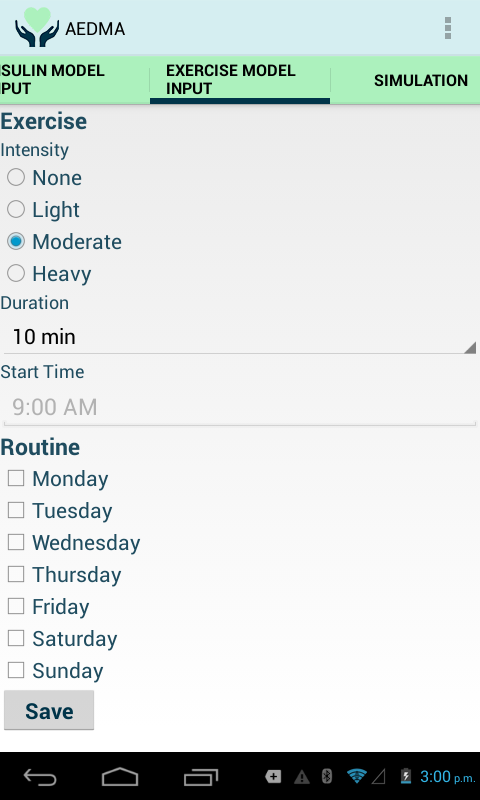
\includegraphics[width=0.17\textwidth]{Figs/Pantalla3_AEDMA}     &        
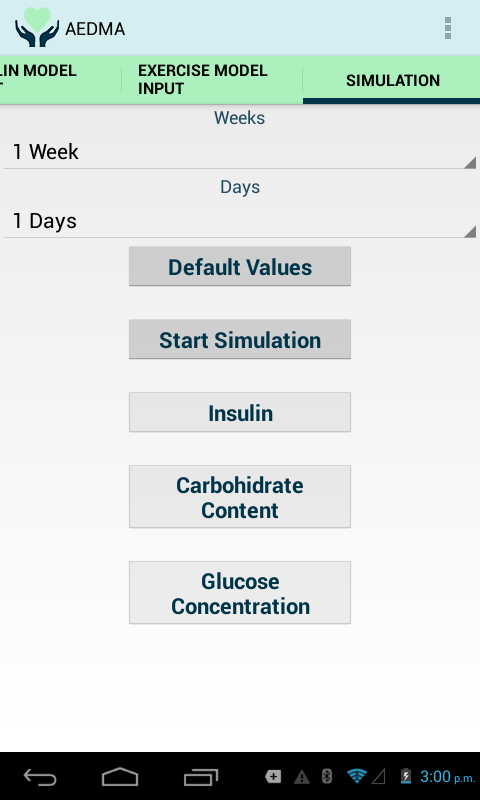
\includegraphics[width=0.17\textwidth]{Figs/Pantalla4_AEDMA} \\ 
1 & 2 & 3 & 4 & 5 \\
          \end{tabular}
\end{center}
\end{block} 
\end{frame}

\begin{frame}{\citetitle{MarcoNuno_Revista_2020_10_00} (4)}
\begin{block}{Validation of insulin and meal intake models } 
\begin{columns}
\begin{column}{0.45\textwidth}


Simulation duration: 5 days
\begin{enumerate}
\item Default carbohydrate and insulin doses
\item Default insulin doses but reduce carbohydrate
\item Default carbohydrate but insulin is increased
\item Both insulin increased and carbohydrate reducton
\end{enumerate}

\note[item]{Simulation 1: Glucose peak is close to 195 mg/dL every day of the reported simulation}
\note[item]{Simulation 2: Glucose peak surpasses 175 mg/dL due to the reduction of carbohydrate intake. }
\note[item]{Simulation 3: Glucose peak surpasses 175 mg/dL with the same carbohydrate configuration, but both prolonged and rapid insulin doses are doubled.}
\note[item]{Simulation 4: Combination of exp. 2 (carbohygrate reduction) and exp 3. (insulin doses doubling). }

%Figure 5 shows a glucose concentration plot for a 5-day simulation for each experiment reported in Table 3. In Figure 5a, the maximum glucose peak is close to 195 mg/dL every day of the reported simulation. In contrast, in Figure 5b, the maximum glucose peak surpasses 175 mg/dL due to the reduction of carbohydrate intake. In Figure 5c, the same carbohydrate intake is used, but both prolonged and rapid insulin doses are doubled. It can be shown that glucose levels are lower when compared with the plot of experiment 1, and in Figure 5d, also the carbohydrate intake is reduced to half to validate both meal and insulin models. In both experiments (3 and 4), it can be shown for its corresponding plots that even a risk of hyperglycemia is present due to the high insulin dose.


%La aplicación genera una gráfica de comportamiento de la glucosa a lo largo del tiempo de simulación. Se muestran las gráficas para cuatro casos:
%	\begin{itemize}
%\item Pacientes controlados en cuanto a los niveles de glucosa (a y b)
%\item Pacientes fuera de control debido a la falta de ejercicio y al exceso de carbohidratos (c y d)
%	\end{itemize}
\end{column}
\begin{column}{0.40\textwidth}
\begin{center}
\begin{tabular}{c}
\includegraphics[width=0.43\textwidth]{Figs/Experimento1_AEDMA}     
\includegraphics[width=0.43\textwidth]{Figs/Experimento2_AEDMA}     \\

\includegraphics[width=0.43\textwidth]{Figs/Experimento3_AEDMA}     
\includegraphics[width=0.43\textwidth]{Figs/Experimento4_AEDMA}     \\        
          \end{tabular}
     \end{center}
\end{column}
\end{columns}
\end{block} 
\end{frame}




% Figure 1 shows a simulation using 10 minutes of light exercise. The value of glucose peak after excersive at 9:00 AM is close to 185 mg/DL, but this value is lowered to 180 mg/DL changing the configuration to 30 minuts of light exercise (Figure 2) . 

